\begin{figure}
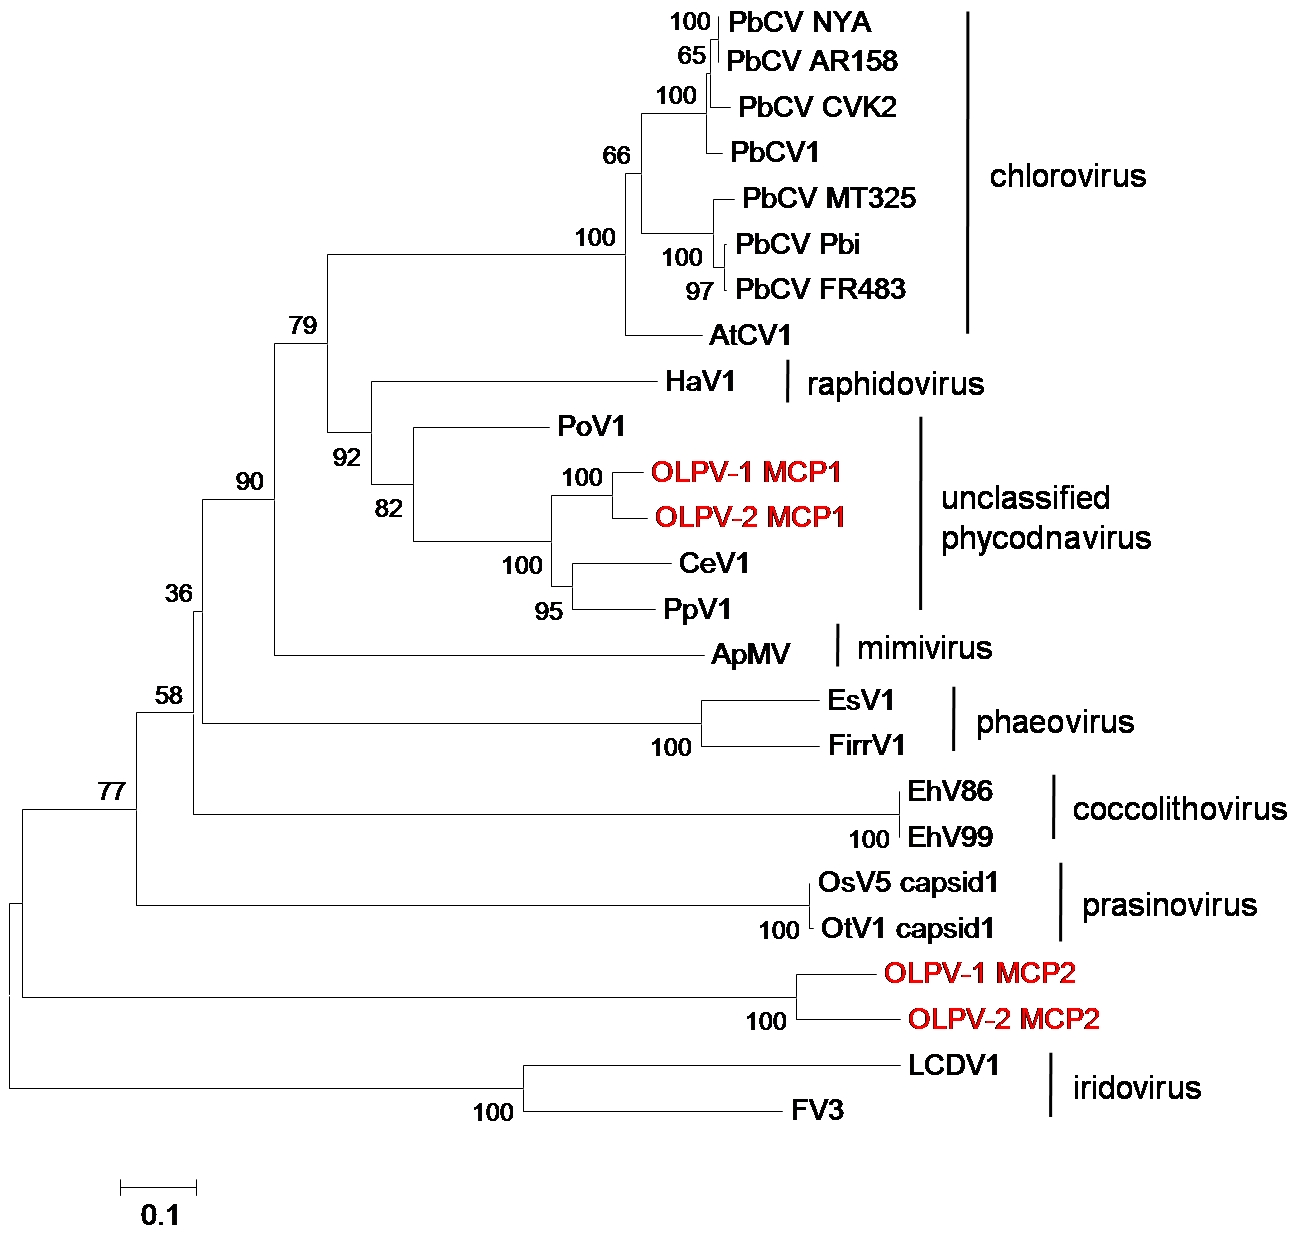
\includegraphics[width=\textwidth]{olv_figures/OLPV_full_mcp.jpg}
\caption[Phylogeny of \acs{OLPV} major capsid protein sequences]{Neighbour-joining tree of major capsid protein amino acid sequences from \ac{OLPV} and  other \acs{NCLDV} sequences from GenBank. 
Abbreviations and accession numbers from top to bottom: PbCV NYA, \emph{Paramecium bursaria} chlorella virus NY2A (ABT14984.1); PbCV AR158, \emph{P. bursaria} chlorella virus AR158 (ABU44077.1); PbCV CVK2, \emph{P. bursaria} chlorella virus CVK2 (BAA35143.1); PbCV1, \emph{P. bursaria} chlorella virus 1(AAA88828.1); PbCV MT325, \emph{P. bursaria} chlorella virus MT325 (ABT14017.1); PbCV Pbi, \emph{P. bursaria} chlorella virus Pbi (AAC27492.1); PbCV FR483, \emph{P. bursaria} chlorella virus FR483 (ABT15755.1); AtCV1, \emph{Acathocystis turfacea} chlorella virus 1 (ABT16414.1); HaV1, \emph{Heterosigma akashiwo} virus 1 (BAE06835.1); PoV, \emph{Pyramimonas orientalis} virus (ABU23714.1); CeV1, \emph{Chrysochromulina ericinia} virus 1 (ABU23712.1); PpV1, \emph{Phaeocystis pouchetii} virus (ABU23715.1); ApMV, \emph{Acathamoeba polyphaga} virus (Q5UQL7.2); EsV1, \emph{Ectocarpus siliculosus} virus (AAK14534.1); FirrV1, \emph{Feldmannia irregularis} virus 1 (AAR26925.1); EhV86, \emph{Emiliania huxleyi} virus 86 (CAI65508.2); EhV99, \emph{E. huxleyi} virus 99 (ABU23713.1); OsV5, \emph{Ostreococcus} virus 5 (ABY27849.1); OtV1, \emph{O. tauri} virus 1 (CAY39653.1); LCDV1, Lymphocystis diseases virus 1(AAC24486.2); FV3, Frog virus 3 (AAT09750.1). 
}
\label{fig:OLPV_full_mcp}

\end{figure}
